\section{Basics}\label{sec_basics}

PEC takes advantage of the photovoltaic\index{photovoltaic} effect, discovered by 
\citet{becquerel1839} in 1839, that occurs at the interface of a semiconductor
and an electrolyte. 
In fact, the first experience showed the occurrence of a photopotential and 
a photocurrent under illumination when a silver electrode, 
covered with an oxide layer, was immersed in an acidic medium and connected 
to a platinum electrode. 
Nonetheless, the first studies focused on the understanding of the interfacial 
processes were performed much later 
\citep{stimming1986,gerischer1966,copeland1942}.

The basics of photoelectrochemistry and application examples are presented in 
the following sections and they are largely described in the literature 
\citep{morrison1980,gerischer1985,memming2008,marcus2006,bard2002,sato1998}. 
Several hypotheses are needed in order to apply the theoretical concepts:  
\begin{itemize}
\item semiconductor are considered to be ideal i.e. crystallized and homogeneous  
\item the dielectric constant of the semiconductor is independent of the light wavelength  
\item the capacity of the Helmholtz layer is greater than the capacitance of the space charge capacitance  
\item the potential drop in the Helmholtz layer is independent of the applied potential and is negligible
\end{itemize}

The hypotheses are rarely fully respected in the case of oxides or passive 
films formed on industrial alloys. Nonetheless, the literature shows that the 
developed models can be applied to non-ideal systems such as oxides 
and passive films.


\subsection{Electronic Band Structure}

Solids are generally classified into three groups: 
conductors\index{conductors}, semiconductors\index{semiconductors} and isolators\index{isolators}. 
Each category can be illustrated with a specific band structure as shown in 
figure~\ref{fig_band_model}. 
Valence and conduction bands correspond to allowed energy states for the electrons. 
The lowest energy level of the conduction band is labeled $E_c$ and the 
highest energy level of the valence band is labeled $E_v$. 
They are separated by a band gap, $E_g$, with no allowed energy states. 
The repartition of the electrons among both bands are described by the position 
of the Fermi Level, $E_F$, which represents the highest energy state that 
can be occupied level at 0K. 
It is equivalent to the electrochemical potential in solid phases.

\begin{figure}[h]
\centering
\begin{circuitikz}[scale=1.0]
\small
\draw[->] (0,-3) -- ++(0,6);
\node[anchor=center, rotate=90] at (-0.25,0) {Electron Energy};

\draw[dashed, thick] (0,0) -- ++(10,0);
\node[draw=none, anchor=south] at (5,0.2) {Fermi Level: $E_F$};

\node[rectangle, minimum height=1.5cm, anchor=south, draw=red, align=center, text width=2cm, fill=red!20] at (2, -0.2) {Conduction Band};
\node[rectangle, minimum height=1.5cm, anchor=north, draw=green, align=center, text width=2cm, fill=green!20] at (2, 0.2) {Valence Band};
\node[rectangle, minimum height=0.4cm, anchor=center, draw=orange, align=center, text width=2cm, fill=orange!20] at (2, 0.0) {};

\node[rectangle, anchor=south, draw=red, align=center, text width=2cm, fill=red!20] at (5, 1.) {Conduction Band};
\node[rectangle, anchor=north, draw=green, align=center, text width=2cm, fill=green!20] at (5, -1.) {Valence Band};

\node[draw=none, anchor=south west, blue] at (9.2,+0.2) {Band Gap: $E_g$};
\draw[<->, thick, blue,] (9,-1.5) -- ++(0,3);
\node[rectangle, anchor=south , draw=red, align=center, text width=2cm, fill=red!20] at (9, 1.5) {Conduction Band};
\node[rectangle, anchor=north , draw=green, align=center, text width=2cm, fill=green!20] at (9, -1.5) {Valence Band};

\end{circuitikz}
\caption{Schematic representation of the electronic band structure \citep{marucco2006-1}: 
a) conductor, b) semiconductor, c) isolator}
\label{fig_band_model}
\end{figure}

The electronic conduction is due to the movement either of the negatively 
charged electrons in the conduction band or of the positively charged holes 
in the valence band or both simultaneously. 
Consequently, the conduction depends on the number of available charge carriers
in the conduction band and in the valence band. 
In conductors, an overlap of the conduction and the valence bands occurs 
which means that the highest allowed energy band is partially filled. 
The distinction between a semiconductor and an isolator is less obvious 
because the conduction depends on the band gap and the energy provided by 
the environment to the electrons from the valence band in order to jump 
into the conduction band.

In semiconductors, charge carriers can be generated by three mechanisms: 
\emph{thermal excitation, photoexcitation and doping} as shown in 
figure~\ref{fig_excitation_carrier}. 
In the case of very low band gaps, thermal excitation can be enough in order 
to eject an electron from the valence band to the conduction band. 
Photoexcitation ejects electrons from the valence band to the conduction 
band when an incident photon, with energy greater than the band gap, is absorbed. 
Doping introduces additional energy level located in between the conduction and 
valence bands.

Doping occurs when the stoichiometry is altered or when impurities are 
introduced in the crystallographic lattice of the semiconductor. 
In the case of n-type semiconductors, the donor energy levels $E_d$ lie just 
under the conduction band. The electrons from the donor levels are ejected by 
thermal excitation. 
Consequently, the majority charge carriers are negatively charged electrons 
in the band conduction. 
Similarly, the acceptor energy levels $E_a$, of p-type semiconductors, 
lie just above the band valence. 
The latter trap electrons from the valence band and therefore create holes. 
Consequently, the majority charge carriers are positively charged holes.

\begin{figure}[h]
\centering
\begin{circuitikz}[scale=1.0]

% Thermal Excitation
\coordinate (XY) at (0,0);
\draw[-Stealth, thick] ($(XY)+(1,0)$) -- ++(0,3);
\draw[color=green] ($(XY)+(0,0)$) -- ++(2,0);
\draw[rectangle, anchor=north , draw=green, fill=green!20] ($(XY)+(0.2,0)$) rectangle ++(1.6,-1);
\draw ($(XY)+(1,-0.5)$) circle [radius=0.3] node {+};
\draw[color=red] ($(XY)+(0,3)$) -- ++(2,0);
\draw[rectangle, anchor=north , draw=red, fill=red!20] ($(XY)+(0.2,3)$) rectangle ++(1.6,1);
\draw ($(XY)+(1,3.5)$) circle [radius=0.3] node {-};
\node[anchor=west] at ($(XY)+(2,0)$) {$E_v$};
\node[anchor=west] at ($(XY)+(2,3)$) {$E_c$};
\node[anchor=center, align=center] at ($(XY)+(1, -2)$) {a) Thermal\\Excitation};

% Photoexcitation
\coordinate (XY) at (3,0);
\draw[-Stealth, thick] ($(XY)+(1,0)$) -- ++(0,3);
\draw[color=green] ($(XY)+(0,0)$) -- ++(2,0);
\draw[rectangle, anchor=north , draw=green, fill=green!20] ($(XY)+(0.2,0)$) rectangle ++(1.6,-1);
\draw ($(XY)+(1,-0.5)$) circle [radius=0.3] node {+};
\draw[color=red] ($(XY)+(0,3)$) -- ++(2,0);
\draw[rectangle, anchor=north , draw=red, fill=red!20] ($(XY)+(0.2,3)$) rectangle ++(1.6,1);
\draw ($(XY)+(1,3.5)$) circle [radius=0.3] node {-};
\node[anchor=west] at ($(XY)+(2,0)$) {$E_v$};
\node[anchor=west] at ($(XY)+(2,3)$) {$E_c$};
\node[anchor=center, align=center] at ($(XY)+(1, -2)$) {b) Photoexcitation};

% Doping
\coordinate (XY) at (6,0);
\draw[color=green] ($(XY)+(0,0)$) -- ++(1.5,0);
\draw[rectangle, anchor=north , draw=green, fill=green!20] ($(XY)+(0.2,0)$) rectangle ++(1.1,-1);
\draw[color=red] ($(XY)+(0,3)$) -- ++(1.5,0);
\draw[rectangle, anchor=north , draw=red, fill=red!20] ($(XY)+(0.2,3)$) rectangle ++(1.1,1);
\node[anchor=north, align=center] at ($(XY)+(0.75, -1)$) {n-type};
\draw[color=black] ($(XY)+(0,2)$) -- ++(1.5,0);
\draw[-Stealth, thick] ($(XY)+(0.5,2.5)$) -- ++(0,0.5);
\draw[-Stealth, thick] ($(XY)+(1,2.5)$) -- ++(0,0.5);
\node[draw, anchor=south, align=center, circle, minimum size=0.2pt, inner sep=0] at ($(XY)+(0.5,2)$) {+};
\node[draw, anchor=south, align=center, circle, minimum size=0.2pt, inner sep=0] at ($(XY)+(1,2)$) {+};
\node[draw, anchor=south, align=center, circle, minimum size=0.2pt, inner sep=2] at ($(XY)+(0.5,3)$) {-};
\node[draw, anchor=south, align=center, circle, minimum size=0.2pt, inner sep=2] at ($(XY)+(1,3)$) {-};
\node[anchor=west] at ($(XY)+(1.5,0)$) {$E_v$};
\node[anchor=west] at ($(XY)+(1.5,3)$) {$E_c$};
\node[anchor=west] at ($(XY)+(1.5,2.0)$) {$E_d$};

\node[anchor=center, align=center] at ($(XY)+(2, -2)$) {c) Doping};

\coordinate (XY) at (8.2,0);
\draw[color=green] ($(XY)+(0,0)$) -- ++(1.5,0);
\draw[rectangle, anchor=north , draw=green, fill=green!20] ($(XY)+(0.2,0)$) rectangle ++(1.1,-1);
\draw[color=red] ($(XY)+(0,3)$) -- ++(1.5,0);
\draw[rectangle, anchor=north , draw=red, fill=red!20] ($(XY)+(0.2,3)$) rectangle ++(1.1,1);
\node[anchor=north, align=center] at ($(XY)+(0.75, -1)$) {p-type};
\draw[color=black] ($(XY)+(0,1)$) -- ++(1.5,0);
\draw[-Stealth, thick] ($(XY)+(0.5,0.0)$) -- ++(0,1);
\draw[-Stealth, thick] ($(XY)+(1,0.0)$) -- ++(0,1);
\node[draw, anchor=south, align=center, circle, minimum size=0.2pt, inner sep=0] at ($(XY)+(0.5,-0.5)$) {+};
\node[draw, anchor=south, align=center, circle, minimum size=0.2pt, inner sep=0] at ($(XY)+(1,-0.5)$) {+};
\node[draw, anchor=south, align=center, circle, minimum size=0.2pt, inner sep=2] at ($(XY)+(0.5,1)$) {-};
\node[draw, anchor=south, align=center, circle, minimum size=0.2pt, inner sep=2] at ($(XY)+(1,1)$) {-};
\node[anchor=west] at ($(XY)+(1.5,0)$) {$E_v$};
\node[anchor=west] at ($(XY)+(1.5,3)$) {$E_c$};
\node[anchor=west] at ($(XY)+(1.5,1)$) {$E_a$};
\end{circuitikz}
\caption{Schematic representation of the mechanisms generating charge carriers in semiconductors \citep{finklea1983-1}: 
a) thermal excitation, b) photoexcitation, c) doping}
\label{fig_excitation_carrier}
\end{figure}

The Fermi level $E_F$ in intrinsic semiconductors is located at the mid-gap. 
The n-type and p-type doping shift the Fermi level towards band edges 
$E_c$ and $E_v$, respectively. 
The figure~\ref{fig_fermi_position} shows the position of the Fermi level 
with respect to the semiconductor type.

\begin{figure}[H]
\centering
\begin{circuitikz}[scale=1.0]
% Intrinsic
\coordinate (XY) at (0,0);
\draw[color=green] ($(XY)+(0,0)$) -- ++(2,0);
\draw[rectangle, anchor=north , draw=green, fill=green!20] ($(XY)+(0.2,0)$) rectangle ++(1.6,-1);
\draw[color=red] ($(XY)+(0,3)$) -- ++(2,0);
\draw[rectangle, anchor=north , draw=red, fill=red!20] ($(XY)+(0.2,3)$) rectangle ++(1.6,1);
\draw[color=black, dashed, thick] ($(XY)+(0,1.5)$) -- ++(2,0);
\node[anchor=west] at ($(XY)+(2,0)$) {$E_v$};
\node[anchor=west] at ($(XY)+(2,3)$) {$E_c$};
\node[anchor=west] at ($(XY)+(2,1.5)$) {$E_F$};
\node[anchor=center, align=center] at ($(XY)+(1, -2)$) {a) Intrinsic};

% n-type
\coordinate (XY) at (4,0);
\draw[color=green] ($(XY)+(0,0)$) -- ++(2,0);
\draw[rectangle, anchor=north , draw=green, fill=green!20] ($(XY)+(0.2,0)$) rectangle ++(1.6,-1);
\draw[color=red] ($(XY)+(0,3)$) -- ++(2,0);
\draw[rectangle, anchor=north , draw=red, fill=red!20] ($(XY)+(0.2,3)$) rectangle ++(1.6,1);
\draw[color=black, dashed, thick] ($(XY)+(0,2.5)$) -- ++(2,0);
\draw[color=black,  thick] ($(XY)+(0,2.0)$) -- ++(2,0);
\node[anchor=west] at ($(XY)+(2,0)$) {$E_v$};
\node[anchor=west] at ($(XY)+(2,3)$) {$E_c$};
\node[anchor=west] at ($(XY)+(2,2.5)$) {$E_F$};
\node[anchor=west] at ($(XY)+(2,2.0)$) {$E_d$};
\node[anchor=center, align=center] at ($(XY)+(1, -2)$) {b) n-type};

% p-type
\coordinate (XY) at (8,0);
\draw[color=green] ($(XY)+(0,0)$) -- ++(2,0);
\draw[rectangle, anchor=north , draw=green, fill=green!20] ($(XY)+(0.2,0)$) rectangle ++(1.6,-1);
\draw[color=red] ($(XY)+(0,3)$) -- ++(2,0);
\draw[rectangle, anchor=north , draw=red, fill=red!20] ($(XY)+(0.2,3)$) rectangle ++(1.6,1);
\draw[color=black, dashed, thick] ($(XY)+(0,0.5)$) -- ++(2,0);
\draw[color=black,  thick] ($(XY)+(0,1.0)$) -- ++(2,0);
\node[anchor=west] at ($(XY)+(2,0)$) {$E_v$};
\node[anchor=west] at ($(XY)+(2,3)$) {$E_c$};
\node[anchor=west] at ($(XY)+(2,0.5)$) {$E_F$};
\node[anchor=west] at ($(XY)+(2,1.0)$) {$E_a$};
\node[anchor=center, align=center] at ($(XY)+(1, -2)$) {b) p-type};

\end{circuitikz}
\caption{Schematic representation of the Fermi level with respect to the 
semiconduction type \citep{finklea1983}: a) intrinsic, b) n-type, c) p-type.}
\label{fig_fermi_position}
\end{figure}




\subsection{Semiconductor/electrolyte interface in dark condition}
A potential gradient occurs when a semiconductor comes into contact with an 
electrolyte as shown in figure~\ref{fig_interface_potential}.
The position of the Fermi level in the electrolyte with respect to the 
conduction and valence band edges leads to three different situations after 
a transient charge transfer. 
The flat band situation occurs when the Fermi level in the electrolyte 
matches the Fermi level in the semiconductor. 
Consequently, there is no potential gradient in the semiconductor. 
In a case of Fermi level mismatch, a band bending occurs in the semiconductor 
near the semiconductor/electrolyte interface. 
The band bending leads to either depletion or accumulation of majority 
charge carriers near the semiconductor/electrolyte interface. 
The spatial extension of the depletion/accumulation zone is called space 
charge as shown in figure~\ref{fig_space_charge_depletion}.

\begin{figure}[h]
\centering
\begin{circuitikz}[scale=1.0]
\coordinate (O) at (0,0);
\coordinate (X_axis) at (8,0);
\coordinate (Phi_axis) at (0,4);
\coordinate (Phi_sc_x) at (0,0);
\coordinate (Phi_sc_y) at (0,3.5);
\coordinate (Phi_sc) at ($(Phi_sc_x)+(Phi_sc_y)$);
\coordinate (Phi_el_x) at (8,0);
\coordinate (Phi_el_y) at ($(Phi_sc_y)+(0,-1)$);
\coordinate (Phi_el) at ($(Phi_el_x)+(Phi_el_y)$);
\coordinate (wh_x) at ($(Phi_el_x)+(-2,0)$);
\coordinate (wh_y) at (0,0);
\coordinate (wh) at ($(wh_x)+(wh_y)$);
\coordinate (wsc_x) at ($(Phi_sc_x)+(3,0)$);
\coordinate (wsc_y) at (0,0);
\coordinate (wsc) at ($(wsc_x)+(wsc_y)$);
\coordinate (ix) at ($(wh_x)!0.5!(wsc_x)$);
\coordinate (iy) at (0,0);
\coordinate (i) at ($(ix)+(iy)$);

\draw[-Stealth] (O) -- (X_axis) node[at end, below] {$X$};
\draw[-Stealth] (O) -- (Phi_axis) node[midway, left, anchor=south, rotate=90] {Potential};

\draw (Phi_sc) -- ++(8,0) node[at start, left] {$\Phi_{sc}$} ;
\draw (Phi_el) -- ($(wh_x)+(Phi_el_y)$) node[near start, below] {$\Phi_{el}$};

\draw[blue] (wh) -- ($(wh_x)+(Phi_sc_y)$) node[at start,below] {$w_H$};
\draw[red] (wsc) -- ($(wsc_x)+(Phi_sc_y)$) node[at start, below] {$w_{sc}$};
\draw[black] (i) -- ($(ix)+(Phi_sc_y)$) node[at start, below] {$0$};

\draw ($(wh_x)+(Phi_el_y)$) to[in=-5, out=175] ($(Phi_sc)+(3,0)$);
\draw[Stealth-Stealth, thick] ($(Phi_el)+(-0.5,0)$) -- ($(Phi_el)+(-0.5,1)$) node[right, midway] {$\Delta \Phi _{sc/el}$};

\end{circuitikz}
\caption{Potential gradient at semiconductor/electrolyte interface 
\citep{marcus2006}. $\Phi_{sc}$ and $\Phi_{el}$ correspond to the 
potentials of the semiconductor and the electrolyte, respectively. 
$\Delta Phi _{sc/el}$ corresponds to the potential difference between 
the semiconductor and the electrolyte. $w_{sc}$ and $w_{H}$ correspond to 
the widths of the space charge and the electrical double layer, 
respectively.}
\label{fig_interface_potential}
\end{figure}

\begin{figure}[H]
\centering
\begin{circuitikz}[scale=1.0]

% left n-type
\coordinate (Ox) at (-0.5,0);
\coordinate (Oy) at (0,0);
\coordinate (O) at ($(Ox)+(Oy)$);
\coordinate (xlen) at (-6,0);
\coordinate (ylen) at (+0,4);
\coordinate (wsc_x) at ($(Ox)+(-4,0)$);
\coordinate (wsc_y) at ($(Oy)+(ylen)$);
\coordinate (Ev_x) at ($(Ox)+(xlen)$);
\coordinate (Ev_y) at ($(Oy)+(0,1)$);
\coordinate (Ev) at ($(Ev_x)+(Ev_y)$);
\coordinate (Ec_x) at ($(Ox)+(xlen)$);
\coordinate (Ec_y) at ($(Ev_y)+(0,2)$);
\coordinate (Ec) at ($(Ec_x)+(Ec_y)$);
\coordinate (Ef_x) at ($(Ox)+(xlen)$);
\coordinate (Ef_y) at ($(Ec_y)+(0,-0.5)$);
\coordinate (Ef) at ($(Ef_x)+(Ef_y)$);

\draw[-Stealth] (O) -- ($(O)+(xlen)$) node[at end, below] {$x$};
\draw[-Stealth] (O) -- ($(O)+(ylen)$) node[at end, left] {$E$};
\draw[blue, dashed] (wsc_x) -- ($(wsc_x)+(ylen)$) node[at start, below] {$w_{sc}$};
\draw[red] (Ec) -- ($(wsc_x)+(Ec_y)$) node [at start, left] {$E_c$};
\draw[red] ($(wsc_x)+(Ec_y)$) to[in=-165, out=0] ($(Ox)+(Ec_y)+(0,0.5)$);
\draw[green] (Ev) -- ($(wsc_x)+(Ev_y)$) node [at start, left] {$E_v$};
\draw[green] ($(wsc_x)+(Ev_y)$) to[in=-165, out=0] ($(Ox)+(Ev_y)+(0,0.5)$);
\draw[dashed] (Ef) -- ($(Ox)+(Ef_y)$) node [at start, left] {$E_F$};
\draw[rectangle, text width=2cm, blue] ($(wsc_x)+(Ec_y)+(0, 0.5)$) node[anchor=west] {\small Space charge $e^-$ depletion};
\draw[blue, dashed] (wsc_x) -- ($(wsc_x)+(ylen)$);
\node[anchor=north, align=center, yshift=-0.5cm] at ($(Ox)!0.5!(xlen)$) {a) n-type};
\draw[Stealth-Stealth, blue, thick] ($(wsc_x)+(Ev_y)+(0.2,0)$) -- ($(wsc_x)+(Ec_y)+(0.2,0)$) node[midway, right] {$E_g$};

% right p-type
\coordinate (Ox) at (0.5,0);
\coordinate (Oy) at (0,0);
\coordinate (O) at ($(Ox)+(Oy)$);
\coordinate (xlen) at (+6,0);
\coordinate (ylen) at (+0,4);
\coordinate (wsc_x) at ($(Ox)+(4,0)$);
\coordinate (wsc_y) at ($(Oy)+(ylen)$);
\coordinate (Ev_x) at ($(Ox)+(xlen)$);
\coordinate (Ev_y) at ($(Oy)+(0,1)$);
\coordinate (Ev) at ($(Ev_x)+(Ev_y)$);
\coordinate (Ec_x) at ($(Ox)+(xlen)$);
\coordinate (Ec_y) at ($(Ev_y)+(0,2)$);
\coordinate (Ec) at ($(Ec_x)+(Ec_y)$);
\coordinate (Ef_x) at ($(Ox)+(xlen)$);
\coordinate (Ef_y) at ($(Ev_y)+(0,0.5)$);
\coordinate (Ef) at ($(Ef_x)+(Ef_y)$);

\draw[-Stealth] (O) -- ($(O)+(xlen)$) node[at end, below] {$x$};
\draw[-Stealth] (O) -- ($(O)+(ylen)$) node[at end, right] {$E$};
\draw[blue, dashed] (wsc_x) -- ($(wsc_x)+(ylen)$) node[at start, below] {$w_{sc}$};
\draw[red] (Ec) -- ($(wsc_x)+(Ec_y)$) node [at start, right] {$E_c$};
\draw[red] ($(wsc_x)+(Ec_y)$) to[in=15, out=180] ($(Ox)+(Ec_y)+(0,-0.5)$);
\draw[green] (Ev) -- ($(wsc_x)+(Ev_y)$) node [at start, right] {$E_v$};
\draw[green] ($(wsc_x)+(Ev_y)$) to[in=15, out=180] ($(Ox)+(Ev_y)+(0,-0.5)$);
\draw[dashed] (Ef) -- ($(Ox)+(Ef_y)$) node [at start, right] {$E_F$};
\draw[rectangle, text width=2cm, blue] ($(wsc_x)+(Ec_y)+(0, 0.5)$) node[anchor=east] {\small Space charge $h^{\bullet}$ depletion};
\node[anchor=north, align=center, yshift=-0.5cm] at ($(Ox)!0.5!(xlen)$) {b) p-type};
\draw[Stealth-Stealth, blue, thick] ($(wsc_x)+(Ev_y)+(-0.2,0)$) -- ($(wsc_x)+(Ec_y)+(-0.2,0)$) node[midway, left] {$E_g$};

\end{circuitikz}
\caption{Schematic representation of the space charge in depletion of majority charge carriers for 
a semiconductor in contact with an electrolyte \citep{memming2008-1,bard2002-1}:
 a) n-type, b) p-type.}
\label{fig_space_charge_depletion}
\end{figure}

Depletion and accumulation as well as band bending can be obtained 
by polarizing the semiconductor. 
As long as the hypothesis described in the introduction paragraph stand, 
the polarization does not modify the surface band edges $E_{cs}$ and $E_{vs}$. 
Consequently, the polarization will only alter the band bending in the space 
charge. 
Depending on the applied potential, $U$, with respect to the flat band 
potential, $U_fb$, three different situations will occur as shown in 
figure~\ref{fig_band_bending}:
\begin{itemize}
\item $U = U_{fb}$: flat band situation no matter the semiconductor type
\item $U > U_{fb}$: depletion (accumulation) in a case of n-type (p-type) semiconductor  
\item $U < U_{fb}$: accumulation (depletion) in a case of n-type (p-type) semiconductor
\end{itemize}

Without illumination, cathodic (anodic) currents are favored in a case of 
accumulation of electrons (holes) for an n-type (p-type) semiconductor. 
In fact, the majority charge carriers of n-type (p-type) semiconductors are 
electrons (holes). 
Reciprocally, anodic (cathodic) currents are not favored in a case of 
depletion of electrons (holes) for an n-type (p-type) semiconductor. 
The junction between a semiconductor and an electrolyte acts like a Schottky diode.

\begin{figure}[H]
\centering
\documentclass{standalone}

\usepackage{tikz}
\usepackage{circuitikz}
\usetikzlibrary{shadings,decorations.pathmorphing,arrows,calc,patterns,patterns.meta}
\usepackage{graphicx}

\begin{document}


\begin{circuitikz}[scale=1.0]
%U = ufb
% left n-type
\coordinate (Ox) at (-1,0);
\coordinate (Oy) at (0,0);
\coordinate (O) at ($(Ox)+(Oy)$);
\coordinate (xlen) at (-6,0);
\coordinate (ylen) at (+0,4);
\coordinate (wsc_x) at ($(Ox)+(-4,0)$);
\coordinate (wsc_y) at ($(Oy)+(ylen)$);
\coordinate (wsc) at ($(wsc_x)+(wsc_y)$);
\coordinate (Ev_x) at ($(Ox)+(xlen)$);
\coordinate (Ev_y) at ($(Oy)+(0,1)$);
\coordinate (Ev) at ($(Ev_x)+(Ev_y)$);
\coordinate (Ec_x) at ($(Ox)+(xlen)$);
\coordinate (Ec_y) at ($(Ev_y)+(0,2)$);
\coordinate (Ec) at ($(Ec_x)+(Ec_y)$);
\coordinate (Ef_x) at ($(Ox)+(xlen)$);
\coordinate (Ef_y) at ($(Ec_y)+(0,-0.25)$);
\coordinate (Ef) at ($(Ef_x)+(Ef_y)$);

\draw[-Stealth] (O) -- ($(O)+(xlen)$) node[at end, below] {$x$};
\draw[-Stealth] (O) -- ($(O)+(ylen)$) node[at end, left] {$E$};
\draw[blue, dashed] (wsc_x) -- ($(wsc_x)+(ylen)$) node[at start, below] {$w_{sc}$};
\draw[red] (Ec) -- ($(wsc_x)+(Ec_y)$) node [at start, left] {$E_c$};
\draw[red] ($(wsc_x)+(Ec_y)$) -- ($(Ox)+(Ec_y)+(0,0.0)$);
\draw[green] (Ev) -- ($(wsc_x)+(Ev_y)$) node [at start, left] {$E_v$};
\draw[green] ($(wsc_x)+(Ev_y)$) -- ($(Ox)+(Ev_y)+(0,0.0)$);
\draw[dashed] (Ef) -- ($(Ox)+(Ef_y)$) node [at start, left, below] {$E_F$};
\draw[Stealth-Stealth, blue, thick] ($(wsc_x)+(Ev_y)+(0.2,0)$) -- ($(wsc_x)+(Ec_y)+(0.2,0)$) node[midway, right] {$E_g$};

% % right p-type
\coordinate (Ox) at (1,0);
\coordinate (Oy) at (0,0);
\coordinate (O) at ($(Ox)+(Oy)$);
\coordinate (xlen) at (+6,0);
\coordinate (ylen) at (+0,4);
\coordinate (wsc_x) at ($(Ox)+(4,0)$);
\coordinate (wsc_y) at ($(Oy)+(0,0)$);
\coordinate (Ev_x) at ($(Ox)+(xlen)$);
\coordinate (Ev_y) at ($(Oy)+(0,1)$);
\coordinate (Ev) at ($(Ev_x)+(Ev_y)$);
\coordinate (Ec_x) at ($(Ox)+(xlen)$);
\coordinate (Ec_y) at ($(Ev_y)+(0,2)$);
\coordinate (Ec) at ($(Ec_x)+(Ec_y)$);
\coordinate (Ef_x) at ($(Ox)+(xlen)$);
\coordinate (Ef_y) at ($(Ev_y)+(0,0.25)$);
\coordinate (Ef) at ($(Ef_x)+(Ef_y)$);

\draw[-Stealth] (O) -- ($(O)+(xlen)$) node[at end, below] {$x$};
\draw[-Stealth] (O) -- ($(O)+(ylen)$) node[at end, right] {$E$};
\draw[blue, dashed] (wsc_x) -- ($(wsc_x)+(ylen)$) node[at start, below] {$w_{sc}$};
\draw[red] (Ec) -- ($(wsc_x)+(Ec_y)$) node [at start, right] {$E_c$};
\draw[red] ($(wsc_x)+(Ec_y)$) -- ($(Ox)+(Ec_y)+(0,+0.0)$);
\draw[green] (Ev) -- ($(wsc_x)+(Ev_y)$) node [at start, right] {$E_v$};
\draw[green] ($(wsc_x)+(Ev_y)$) -- ($(Ox)+(Ev_y)+(0,+0.0)$);
\draw[dashed] (Ef) -- ($(Ox)+(Ef_y)$) node [at start, right, above] {$E_F$};
\draw[Stealth-Stealth, blue, thick] ($(wsc_x)+(Ev_y)+(-0.2,0)$) -- ($(wsc_x)+(Ec_y)+(-0.2,0)$) node[midway, left] {$E_g$};

\node at ($(Oy)+(ylen)+(0,-0.5)$) {$U=U_{fb}$};

%U > ufb
% left n-type
\coordinate (Ox) at (-1,0);
\coordinate (Oy) at (0,-6);
\coordinate (O) at ($(Ox)+(Oy)$);
\coordinate (xlen) at (-6,0);
\coordinate (ylen) at (+0,4);
\coordinate (wsc_x) at ($(Ox)+(-4,0)$);
\coordinate (wsc_y) at ($(Oy)+(0,0)$);
\coordinate (wsc) at ($(wsc_x)+(wsc_y)$);
\coordinate (Ev_x) at ($(Ox)+(xlen)$);
\coordinate (Ev_y) at ($(Oy)+(0,1)$);
\coordinate (Ev) at ($(Ev_x)+(Ev_y)$);
\coordinate (Ec_x) at ($(Ox)+(xlen)$);
\coordinate (Ec_y) at ($(Ev_y)+(0,2)$);
\coordinate (Ec) at ($(Ec_x)+(Ec_y)$);
\coordinate (Ef_x) at ($(Ox)+(xlen)$);
\coordinate (Ef_y) at ($(Ec_y)+(0,-0.25)$);
\coordinate (Ef) at ($(Ef_x)+(Ef_y)$);

\draw[-Stealth] (O) -- ($(O)+(xlen)$) node[at end, below] {$x$};
\draw[-Stealth] (O) -- ($(O)+(ylen)$) node[at end, left] {$E$};
\draw[blue, dashed] (wsc) -- ($(wsc)+(ylen)$) node[at start, below] {$w_{sc}$};
\draw[red] (Ec) -- ($(wsc_x)+(Ec_y)$) node [at start, left] {$E_c$};
\draw[red] ($(wsc_x)+(Ec_y)$) to[in=-165, out=0] ($(Ox)+(Ec_y)+(0,0.5)$);
\draw[green] (Ev) -- ($(wsc_x)+(Ev_y)$) node [at start, left] {$E_v$};
\draw[green] ($(wsc_x)+(Ev_y)$) to[in=-165, out=0] ($(Ox)+(Ev_y)+(0,0.5)$);
\draw[dashed] (Ef) -- ($(Ox)+(Ef_y)$) node [at start, left, below] {$E_F$};
\draw[rectangle, text width=2cm, blue] ($(wsc_x)+(Ec_y)+(0, 0.5)$) node[anchor=west] {\small $e^-$ depletion};
\draw[Stealth-Stealth, blue, thick] ($(wsc_x)+(Ev_y)+(0.2,0)$) -- ($(wsc_x)+(Ec_y)+(0.2,0)$) node[midway, right] {$E_g$};

% right p-type
\coordinate (Ox) at (1,0);
\coordinate (Oy) at (0,-6);
\coordinate (O) at ($(Ox)+(Oy)$);
\coordinate (xlen) at (+6,0);
\coordinate (ylen) at (+0,4);
\coordinate (wsc_x) at ($(Ox)+(4,0)$);
\coordinate (wsc_y) at ($(Oy)+(0,0)$);
\coordinate (wsc) at ($(wsc_x)+(wsc_y)$);
\coordinate (Ev_x) at ($(Ox)+(xlen)$);
\coordinate (Ev_y) at ($(Oy)+(0,1)$);
\coordinate (Ev) at ($(Ev_x)+(Ev_y)$);
\coordinate (Ec_x) at ($(Ox)+(xlen)$);
\coordinate (Ec_y) at ($(Ev_y)+(0,2)$);
\coordinate (Ec) at ($(Ec_x)+(Ec_y)$);
\coordinate (Ef_x) at ($(Ox)+(xlen)$);
\coordinate (Ef_y) at ($(Ev_y)+(0,0.25)$);
\coordinate (Ef) at ($(Ef_x)+(Ef_y)$);

\draw[-Stealth] (O) -- ($(O)+(xlen)$) node[at end, below] {$x$};
\draw[-Stealth] (O) -- ($(O)+(ylen)$) node[at end, right] {$E$};
\draw[blue, dashed] (wsc) -- ($(wsc)+(ylen)$) node[at start, below] {$w_{sc}$};
\draw[red] (Ec) -- ($(wsc_x)+(Ec_y)$) node [at start, right] {$E_c$};
\draw[red] ($(wsc_x)+(Ec_y)$) to[in=-15, out=180] ($(Ox)+(Ec_y)+(0,+0.5)$);
\draw[green] (Ev) -- ($(wsc_x)+(Ev_y)$) node [at start, right] {$E_v$};
\draw[green] ($(wsc_x)+(Ev_y)$) to[in=-15, out=180] ($(Ox)+(Ev_y)+(0,+0.5)$);
\draw[dashed] (Ef) -- ($(Ox)+(Ef_y)$) node [at start, right, above] {$E_F$};
\draw[rectangle, text width=3.0cm, blue] ($(wsc_x)+(Ec_y)+(0, 0.5)$) node[anchor=east] {\small $h^{\bullet}$ accumulation};
\draw[Stealth-Stealth, blue, thick] ($(wsc_x)+(Ev_y)+(-0.2,0)$) -- ($(wsc_x)+(Ec_y)+(-0.2,0)$) node[midway, left] {$E_g$};

\node at ($(Oy)+(ylen)+(0,-0.5)$) {$U>U_{fb}$};

%U < Ufb
% left n-type
\coordinate (Ox) at (-1,0);
\coordinate (Oy) at (0,-12);
\coordinate (O) at ($(Ox)+(Oy)$);
\coordinate (xlen) at (-6,0);
\coordinate (ylen) at (+0,4);
\coordinate (wsc_x) at ($(Ox)+(-4,0)$);
\coordinate (wsc_y) at ($(Oy)+(0,0)$);
\coordinate (wsc) at ($(wsc_x)+(wsc_y)$);
\coordinate (Ev_x) at ($(Ox)+(xlen)$);
\coordinate (Ev_y) at ($(Oy)+(0,1)$);
\coordinate (Ev) at ($(Ev_x)+(Ev_y)$);
\coordinate (Ec_x) at ($(Ox)+(xlen)$);
\coordinate (Ec_y) at ($(Ev_y)+(0,2)$);
\coordinate (Ec) at ($(Ec_x)+(Ec_y)$);
\coordinate (Ef_x) at ($(Ox)+(xlen)$);
\coordinate (Ef_y) at ($(Ec_y)+(0,-0.25)$);
\coordinate (Ef) at ($(Ef_x)+(Ef_y)$);

\draw[-Stealth] (O) -- ($(O)+(xlen)$) node[at end, below] {$x$};
\draw[-Stealth] (O) -- ($(O)+(ylen)$) node[at end, left] {$E$};
\draw[blue, dashed] (wsc) -- ($(wsc)+(ylen)$) node[at start, below] {$w_{sc}$};
\draw[red] (Ec) -- ($(wsc_x)+(Ec_y)$) node [at start, left] {$E_c$};
\draw[red] ($(wsc_x)+(Ec_y)$) to[in=165, out=0] ($(Ox)+(Ec_y)+(0,-0.5)$);
\draw[green] (Ev) -- ($(wsc_x)+(Ev_y)$) node [at start, left] {$E_v$};
\draw[green] ($(wsc_x)+(Ev_y)$) to[in=165, out=0] ($(Ox)+(Ev_y)+(0,-0.5)$);
\draw[dashed] (Ef) -- ($(Ox)+(Ef_y)$) node [at start, left, below] {$E_F$};
\draw[rectangle, text width=3cm, blue] ($(wsc_x)+(Ec_y)+(0, 0.5)$) node[anchor=west] {\small $e^-$ accumulation};
\node[anchor=north, align=center, yshift=-0.5cm] at ($(Ox)!0.5!(xlen)+(Oy)$) {n-type};
\draw[Stealth-Stealth, blue, thick] ($(wsc_x)+(Ev_y)+(0.2,0)$) -- ($(wsc_x)+(Ec_y)+(0.2,0)$) node[midway, right] {$E_g$};

% right p-type
\coordinate (Ox) at (1,0);
\coordinate (Oy) at (0,-12);
\coordinate (O) at ($(Ox)+(Oy)$);
\coordinate (xlen) at (+6,0);
\coordinate (ylen) at (+0,4);
\coordinate (wsc_x) at ($(Ox)+(4,0)$);
\coordinate (wsc_y) at ($(Oy)+(0,0)$);
\coordinate (wsc) at ($(wsc_x)+(wsc_y)$);
\coordinate (Ev_x) at ($(Ox)+(xlen)$);
\coordinate (Ev_y) at ($(Oy)+(0,1)$);
\coordinate (Ev) at ($(Ev_x)+(Ev_y)$);
\coordinate (Ec_x) at ($(Ox)+(xlen)$);
\coordinate (Ec_y) at ($(Ev_y)+(0,2)$);
\coordinate (Ec) at ($(Ec_x)+(Ec_y)$);
\coordinate (Ef_x) at ($(Ox)+(xlen)$);
\coordinate (Ef_y) at ($(Ev_y)+(0,0.25)$);
\coordinate (Ef) at ($(Ef_x)+(Ef_y)$);

\draw[-Stealth] (O) -- ($(O)+(xlen)$) node[at end, below] {$x$};
\draw[-Stealth] (O) -- ($(O)+(ylen)$) node[at end, right] {$E$};
\draw[blue, dashed] (wsc) -- ($(wsc)+(ylen)$) node[at start, below] {$w_{sc}$};
\draw[red] (Ec) -- ($(wsc_x)+(Ec_y)$) node [at start, right] {$E_c$};
\draw[red] ($(wsc_x)+(Ec_y)$) to[in=15, out=180] ($(Ox)+(Ec_y)+(0,-0.5)$);
\draw[green] (Ev) -- ($(wsc_x)+(Ev_y)$) node [at start, right] {$E_v$};
\draw[green] ($(wsc_x)+(Ev_y)$) to[in=15, out=180] ($(Ox)+(Ev_y)+(0,-0.5)$);
\draw[dashed] (Ef) -- ($(Ox)+(Ef_y)$) node [at start, right, above] {$E_F$};
\draw[rectangle, text width=3.0cm, blue] ($(wsc_x)+(Ec_y)+(0, 0.5)$) node[anchor=east] {\small $h^{\bullet}$ depletion};
\node[anchor=north, align=center, yshift=-0.5cm] at ($(Ox)!0.5!(xlen)+(Oy)$) {p-type};
\draw[Stealth-Stealth, blue, thick] ($(wsc_x)+(Ev_y)+(-0.2,0)$) -- ($(wsc_x)+(Ec_y)+(-0.2,0)$) node[midway, left] {$E_g$};

\node at ($(Oy)+(ylen)+(0,-0.5)$) {$U<U_{fb}$};

\end{circuitikz}

\end{document}


\caption{Schematic representation of the band bending in p-type and n-type 
semiconductors in contact with an electrolyte \citep{memming2008-1, bard2002-1}:
 a) $U = U_{fb}$, b) $U > U_{fb}$, c) $U < U_{fb}$.}
\label{fig_band_bending}

\end{figure}
\clearpage


\subsection{Semiconductor/electrolyte interface under illumination}
The illumination of the semiconductor/electrolyte interface, 
with photons having an energy greater than the band gap, $E_g$, creates 
electron/hole pairs in the semiconductor. 
By applying the adequate potential the pairs can be separated. 
As a consequence, the majority charge carriers are attracted to the 
semiconductor bulk whereas the minority charge carriers are drawn to the 
semiconductor/electrolyte interface where they can be transferred to a RedOx 
species creating an additional current called photocurrent.  

Figure~\ref{fig_photocurrent_generation} illustrates schematically the 
mechanism leading to the creation of a photocurrent. n-type (p-type) 
semiconductors generate anodic (cathodic) photocurrents where the 
electrons (holes) move towards the external circuit whereas the holes (electrons) 
move towards the interface. 
The photocurrent is significant when the semiconductor/electrolyte junction 
is in depletion. 
Figure~\ref{fig_photocurrent_plieth} shows the anodic (cathodic) photocurrent 
for a GaAs n-type (p-type) semiconductor.

Therefore, the applied potential on n-type (p-type) semiconductors is 
greater (lower) than the flat band potential.

\begin{figure}[h]
    \centering
    \documentclass{standalone}

\usepackage{tikz}
\usepackage{circuitikz}
\usetikzlibrary{shadings,decorations.pathmorphing,arrows,calc,patterns,patterns.meta}
\usepackage{graphicx}

\begin{document}


\begin{circuitikz}[scale=1.0]

% left n-type
\coordinate (Ox) at (-2,0);
\coordinate (Oy) at (0,0);
\coordinate (O) at ($(Ox)+(Oy)$);
\coordinate (xlen) at (-5,0);
\coordinate (ylen) at (+0,4);
\coordinate (wsc_x) at ($(Ox)+(-4,0)$);
\coordinate (wsc_y) at ($(Oy)+(ylen)$);
\coordinate (Ev_x) at ($(Ox)+(xlen)$);
\coordinate (Ev_y) at ($(Oy)+(0,1)$);
\coordinate (Ev) at ($(Ev_x)+(Ev_y)$);
\coordinate (Ec_x) at ($(Ox)+(xlen)$);
\coordinate (Ec_y) at ($(Ev_y)+(0,2)$);
\coordinate (Ec) at ($(Ec_x)+(Ec_y)$);
\coordinate (Ef_x) at ($(Ox)+(xlen)$);
\coordinate (Ef_y) at ($(Ec_y)+(0,-0.5)$);
\coordinate (Ef) at ($(Ef_x)+(Ef_y)$);

\draw[-Stealth] (O) -- ($(O)+(xlen)$) node[at end, below] {$x$};
\draw[-Stealth] (O) -- ($(O)+(ylen)$) node[at end, left] {$E$};
\draw[Stealth-Stealth, blue, thick] ($(wsc_x)+(Ev_y)+(0.2,0)$) -- ($(wsc_x)+(Ec_y)+(0.2,0)$) node[midway, right] {$E_g$};
\draw[red] (Ec) -- ($(wsc_x)+(Ec_y)$) node [at start, left] {$E_c$};
\draw[red] ($(wsc_x)+(Ec_y)$) to[in=-165, out=0] ($(Ox)+(Ec_y)+(0,0.5)$);
\draw[green] (Ev) -- ($(wsc_x)+(Ev_y)$) node [at start, left] {$E_v$};
\draw[green] ($(wsc_x)+(Ev_y)$) to[in=-165, out=0] ($(Ox)+(Ev_y)+(0,0.5)$);
\draw[dashed] (Ef) -- ($(Ox)+(Ef_y)$) node [at start, left] {$E_F$};
\node[anchor=north, align=center, yshift=-0.5cm] at ($(Ox)!0.5!(xlen)$) {a) n-type};
\draw[-Stealth, violet, thick] ($(Ox)+(Ev_y)+(-0.7,0.0)$) -- ($(Ox)+(Ec_y)+(-0.7,0.5)$) node[circle, draw, at start, below, inner sep=0] {+} node[inner sep=2,circle, draw, at end, above] {-};
\draw[-Stealth, violet, thick] ($(Ox)+(Ev_y)+(-0.5, -0.1)$) -- ($(Ox)+(Ev_y)+(0.1,0.1)$) ;
\draw[-Stealth, violet, thick] ($(Ox)+(Ec_y)+(-0.9,0.6)$) -- ($(Ox)+(Ec_y)+(-1.5,0.5)$) ;


% right p-type
\coordinate (Ox) at (2,0);
\coordinate (Oy) at (0,0);
\coordinate (O) at ($(Ox)+(Oy)$);
\coordinate (xlen) at (+5,0);
\coordinate (ylen) at (+0,4);
\coordinate (wsc_x) at ($(Ox)+(4,0)$);
\coordinate (wsc_y) at ($(Oy)+(ylen)$);
\coordinate (Ev_x) at ($(Ox)+(xlen)$);
\coordinate (Ev_y) at ($(Oy)+(0,1)$);
\coordinate (Ev) at ($(Ev_x)+(Ev_y)$);
\coordinate (Ec_x) at ($(Ox)+(xlen)$);
\coordinate (Ec_y) at ($(Ev_y)+(0,2)$);
\coordinate (Ec) at ($(Ec_x)+(Ec_y)$);
\coordinate (Ef_x) at ($(Ox)+(xlen)$);
\coordinate (Ef_y) at ($(Ev_y)+(0,0.5)$);
\coordinate (Ef) at ($(Ef_x)+(Ef_y)$);

\draw[-Stealth] (O) -- ($(O)+(xlen)$) node[at end, below] {$x$};
\draw[-Stealth] (O) -- ($(O)+(ylen)$) node[at end, right] {$E$};
\draw[Stealth-Stealth, blue, thick] ($(wsc_x)+(Ev_y)+(-0.2,0)$) -- ($(wsc_x)+(Ec_y)+(-0.2,0)$) node[midway, left] {$E_g$};
\draw[red] (Ec) -- ($(wsc_x)+(Ec_y)$) node [at start, right] {$E_c$};
\draw[red] ($(wsc_x)+(Ec_y)$) to[in=15, out=180] ($(Ox)+(Ec_y)+(0,-0.5)$);
\draw[green] (Ev) -- ($(wsc_x)+(Ev_y)$) node [at start, right] {$E_v$};
\draw[green] ($(wsc_x)+(Ev_y)$) to[in=15, out=180] ($(Ox)+(Ev_y)+(0,-0.5)$);
\draw[dashed] (Ef) -- ($(Ox)+(Ef_y)$) node [at start, right] {$E_F$};
\node[anchor=north, align=center, yshift=-0.5cm] at ($(Ox)!0.5!(xlen)$) {b) p-type};
\draw[-Stealth, violet, thick] ($(Ox)+(Ev_y)+(0.7,-0.5)$) -- ($(Ox)+(Ec_y)+(0.7,0.0)$) node[circle, draw, at start, below, inner sep=0] {+} node[inner sep=2,circle, draw, at end, above] {-};
\draw[-Stealth, violet, thick] ($(Ox)+(Ec_y)+(0.5,0.1)$) -- ($(Ox)+(Ec_y)+(-0.1,-0.1)$) ;
\draw[-Stealth, violet, thick] ($(Ox)+(Ev_y)+(0.9,-0.6)$) -- ($(Ox)+(Ev_y)+(1.5,-0.5)$) ;


\node at ($(0,0)+(ylen)+(0,-0.5)$) {$h\nu > E_g$};
\draw[-Stealth, violet, decorate, decoration={snake, post length=1mm}] ($(0,0)+(ylen)+(-0.2,-0.75)$) -- ($(0,0)+(ylen)+(-1.5,-1.5)$);
\draw[-Stealth, violet, decorate, decoration={snake, post length=1mm}] ($(0,0)+(ylen)+(+0.2,-0.75)$) -- ($(0,0)+(ylen)+(+1.5,-1.5)$);
\node at ($(0,0)+(0,+0.5)$) {Electrolyte};

\end{circuitikz}

\end{document}


    \caption{Schematic representation of the mechanism generating 
    a photocurrent \citep{memming2008-1,bard2002-1}.}
    \label{fig_photocurrent_generation}
\end{figure}

\begin{figure}[h]
    \centering
    \begin{circuitikz}{scale=1}
\node[anchor=south east] at (0,0) {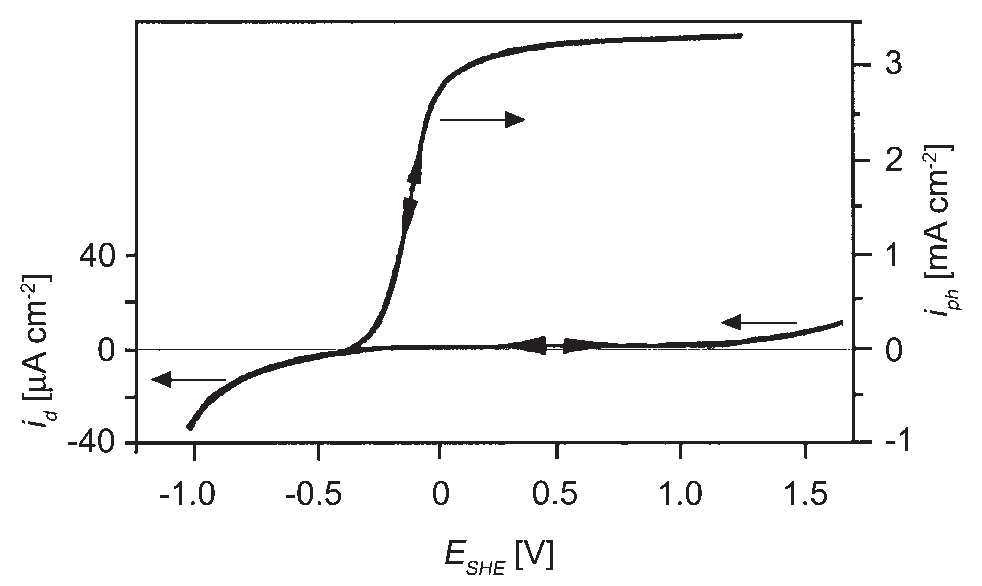
\includegraphics{figures/Plieth_2008-Fig9_10a.png}};
\node[anchor=center] at (-3,0) {a)};
\node[anchor=south west] at (0,0) {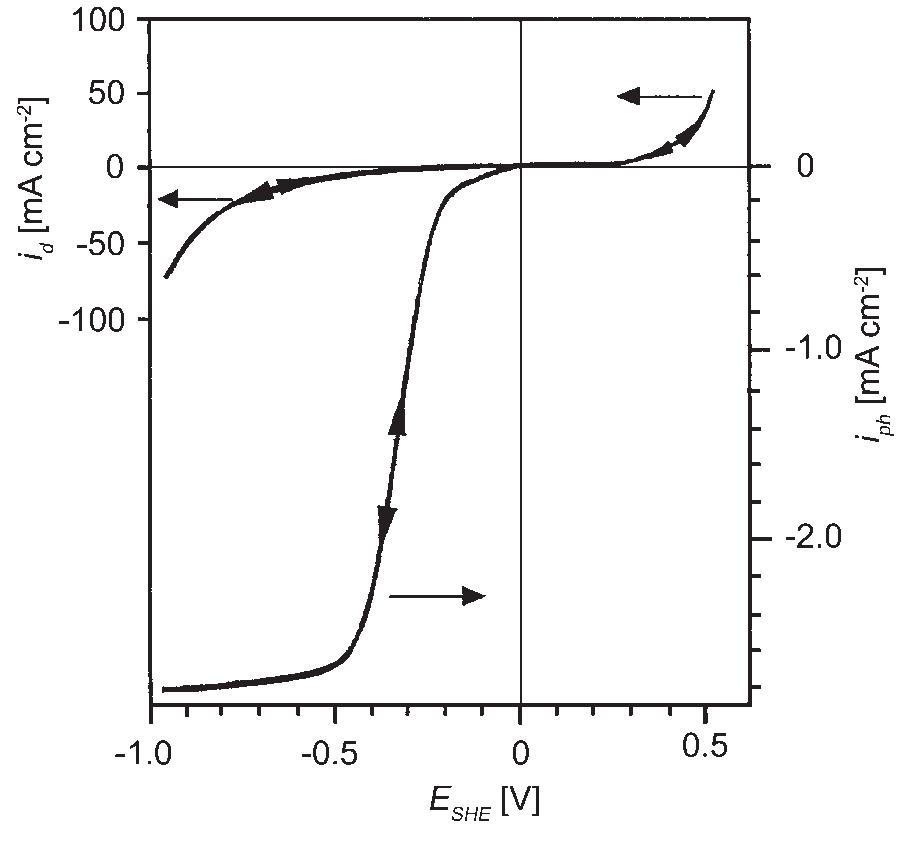
\includegraphics{figures/Plieth_2008-Fig9_10b.png}};
\node[anchor=center] at (3,0) {b)};

\draw[-Stealth, blue, ultra thick] (-4.6,4.1) -- ++(1.5,0.0) node[at end, right, fill=white] {Anodic $i_{ph}$};
\draw[-Stealth, red, ultra thick] (3.5,2.25) -- ++(1.5,0) node[at end, right, fill=white] {Cathodic $i_{ph}$};

\end{circuitikz}
    \caption{Photocurrent density $i_{ph}$ and dark current density 
    $i_d$ with respect to the potential in a case of GaAs semiconductor 
    \citep{plieth2008-1}: a) n-type, b) p-type.}
    \label{fig_photocurrent_plieth}
\end{figure}

\citet{gartner1959} and \citet{butler1977} proposed a simple and robust model for 
describing the photocurrent considering that the recombination of the 
photogenerated electron/hole pairs does not occur in the space charge. 
Therefore, the photocurrent is proportional to the photon flux $\Phi _0$. 
Moreover, the photocurrent depends on the relative ratio between the space 
charge width, $w_{sc}$, the depth of photon penetration given by the inverse 
of the absorption coefficient, $ \alpha $, and the average diffusion length, 
$L_{cc}$, of the minority charge carriers. 
In other words, all absorbed photons generate electron/hole pairs and 
the minority charge carriers are transferred to the electrolyte and 
therefore contribute to the photocurrent whose expression is given 
by the equation~\ref{eq_iph_gartner_butler}.

\begin{equation}
    I_{ph} = \phi _0 \left[ 1 - \frac{\exp (-\alpha _{sc} \cdot w_{sc})}{1+\alpha _{sc} \cdot
    L_{cc}} \right]
    \label{eq_iph_gartner_butler}
\end{equation}

When $\alpha _{sc} \cdot w_{sc} \ll 1$ and $\alpha _{\sc} \cdot L_{cc} \ll 1$, 
the photocurrent is approximated by the 
equation~\ref{eq_iph_gartner_butler_simplified}.

\begin{equation}
    I_{ph} = \phi _0 \cdot \alpha _{\sc} \cdot w_{sc}
    \label{eq_iph_gartner_butler_simplified}
\end{equation}

The expression of the space charge width, $w_{sc}$, in depletion is given 
by the equation~\ref{eq_space_charge_Schottky} according to the Mott-Schottky theory. 
$N_{cc}$ represents the number of majority charge carriers, supposed to be 
equal to the doping, $e$ corresponds to the elementary charge of an electron., 
$U$ represents the applied potential, $U_{fb}$ represent the flat band 
otential, $\epsilon$ and $\epsilon _0$ represent the relative and the 
vacuum permittivity, respectively.

\begin{equation}
    w_{sc} = \sqrt{ \frac{2\epsilon \epsilon _0}{e N_{cc}} (U-U_{fb}-\frac{kT}{e}) }
    \label{eq_space_charge_Schottky}
\end{equation}

The expression of the absorption coefficient $\alpha _{sc}$ with respect to 
the light energy $h\nu$ is shown in equation~\ref{eq_absorption_coef}. 
The value of $n$ depends on the band-band transition type. $n$ takes discreet 
values of 0.5 or 2 when direct or indirect transitions are allowed, respectively.

\begin{equation}
    \alpha _{sc} = const \frac{(h\nu - E_g)^n}{h\nu}
    \label{eq_absorption_coef}
\end{equation}

The complete expression of the photocurrent is therefore given by the 
equation~\ref{eq_iph_substitute_W_alpha}. 
The latter is obtained by substituting the absorption coefficient $\alpha _{sc}$ 
and the space charge width $w_{sc}$ from the 
equation~\ref{eq_iph_gartner_butler_simplified}
by the equations~\ref{eq_space_charge_Schottky} and \ref{eq_absorption_coef}, 
respectively

\begin{equation}
    I_{ph} = \phi _0 \cdot const \frac{(h\nu - E_g)^n}{h\nu}
        \cdot \sqrt{ \frac{2\epsilon \epsilon _0}{e N_{cc}} (U-U_{fb}-\frac{kT}{e}) }
    \label{eq_iph_substitute_W_alpha}
\end{equation}

The linear transform with respect to the energy of the 
equation \ref{eq_iph_substitute_W_alpha} is shown in 
equation~\ref{eq_iph_linear_transform} and it is used for determining 
the band gaps. 
The linear transform with respect to the potential is shown in 
equation~\ref{eq_iph_linear_transform_potential} and it is used for determining 
the semiconduction type, the flat band potential, 
and the number of majority charge carrier.


\begin{equation}
    \left[ \frac{I_{ph} \cdot h\nu}{\phi _0} \right] ^{1/n} = const \cdot (h\nu - E_g)
    \label{eq_iph_linear_transform}
\end{equation}

    \begin{equation}
    I_{ph}^2 = const \cdot (U-U_{fb}-\frac{kT}{e})
    \label{eq_iph_linear_transform_potential}
\end{equation}

